\documentclass[journal,12pt,twocolumn]{IEEEtran}

\usepackage{setspace}
\usepackage{gensymb}
\singlespacing
\usepackage[cmex10]{amsmath}

\usepackage{amsthm}

\usepackage{mathrsfs}
\usepackage{txfonts}
\usepackage{stfloats}
\usepackage{bm}
\usepackage{cite}
\usepackage{cases}
\usepackage{subfig}

\usepackage{longtable}
\usepackage{multirow}

\usepackage{enumitem}
\usepackage{mathtools}
\usepackage{steinmetz}
\usepackage{tikz}
\usepackage{circuitikz}
\usepackage{verbatim}
\usepackage{tfrupee}
\usepackage[breaklinks=true]{hyperref}
\usepackage{graphicx}
\usepackage{tkz-euclide}

\usetikzlibrary{calc,math}
\usepackage{listings}
    \usepackage{color}                                            %%
    \usepackage{array}                                            %%
    \usepackage{longtable}                                        %%
    \usepackage{calc}                                             %%
    \usepackage{multirow}                                         %%
    \usepackage{hhline}                                           %%
    \usepackage{ifthen}                                           %%
    \usepackage{lscape}     
\usepackage{multicol}
\usepackage{chngcntr}

\DeclareMathOperator*{\Res}{Res}

\renewcommand\thesection{\arabic{section}}
\renewcommand\thesubsection{\thesection.\arabic{subsection}}
\renewcommand\thesubsubsection{\thesubsection.\arabic{subsubsection}}

\renewcommand\thesectiondis{\arabic{section}}
\renewcommand\thesubsectiondis{\thesectiondis.\arabic{subsection}}
\renewcommand\thesubsubsectiondis{\thesubsectiondis.\arabic{subsubsection}}


\hyphenation{op-tical net-works semi-conduc-tor}
\def\inputGnumericTable{}                                 %%

\lstset{
%language=C,
frame=single, 
breaklines=true,
columns=fullflexible
}
\begin{document}

\newcommand{\BEQA}{\begin{eqnarray}}
\newcommand{\EEQA}{\end{eqnarray}}
\newcommand{\define}{\stackrel{\triangle}{=}}
\bibliographystyle{IEEEtran}
\raggedbottom
\setlength{\parindent}{0pt}
\providecommand{\mbf}{\mathbf}
\providecommand{\pr}[1]{\ensuremath{\Pr\left(#1\right)}}
\providecommand{\qfunc}[1]{\ensuremath{Q\left(#1\right)}}
\providecommand{\sbrak}[1]{\ensuremath{{}\left[#1\right]}}
\providecommand{\lsbrak}[1]{\ensuremath{{}\left[#1\right.}}
\providecommand{\rsbrak}[1]{\ensuremath{{}\left.#1\right]}}
\providecommand{\brak}[1]{\ensuremath{\left(#1\right)}}
\providecommand{\lbrak}[1]{\ensuremath{\left(#1\right.}}
\providecommand{\rbrak}[1]{\ensuremath{\left.#1\right)}}
\providecommand{\cbrak}[1]{\ensuremath{\left\{#1\right\}}}
\providecommand{\lcbrak}[1]{\ensuremath{\left\{#1\right.}}
\providecommand{\rcbrak}[1]{\ensuremath{\left.#1\right\}}}
\theoremstyle{remark}
\newtheorem{rem}{Remark}
\newcommand{\sgn}{\mathop{\mathrm{sgn}}}
\providecommand{\abs}[1]{\vert#1\vert}
\providecommand{\res}[1]{\Res\displaylimits_{#1}} 
\providecommand{\norm}[1]{\lVert#1\rVert}
%\providecommand{\norm}[1]{\lVert#1\rVert}
\providecommand{\mtx}[1]{\mathbf{#1}}
\providecommand{\mean}[1]{E[ #1 ]}
\providecommand{\fourier}{\overset{\mathcal{F}}{ \rightleftharpoons}}
%\providecommand{\hilbert}{\overset{\mathcal{H}}{ \rightleftharpoons}}
\providecommand{\system}{\overset{\mathcal{H}}{ \longleftrightarrow}}
	%\newcommand{\solution}[2]{\textbf{Solution:}{#1}}
\newcommand{\solution}{\noindent \textbf{Solution: }}
\newcommand{\cosec}{\,\text{cosec}\,}
\providecommand{\dec}[2]{\ensuremath{\overset{#1}{\underset{#2}{\gtrless}}}}
\newcommand{\myvec}[1]{\ensuremath{\begin{pmatrix}#1\end{pmatrix}}}
\newcommand{\mydet}[1]{\ensuremath{\begin{vmatrix}#1\end{vmatrix}}}
\numberwithin{equation}{subsection}
\makeatletter
\@addtoreset{figure}{problem}
\makeatother
\let\StandardTheFigure\thefigure
\let\vec\mathbf
\renewcommand{\thefigure}{\theproblem}
\def\putbox#1#2#3{\makebox[0in][l]{\makebox[#1][l]{}\raisebox{\baselineskip}[0in][0in]{\raisebox{#2}[0in][0in]{#3}}}}
     \def\rightbox#1{\makebox[0in][r]{#1}}
     \def\centbox#1{\makebox[0in]{#1}}
     \def\topbox#1{\raisebox{-\baselineskip}[0in][0in]{#1}}
     \def\midbox#1{\raisebox{-0.5\baselineskip}[0in][0in]{#1}}
\vspace{3cm}
\title{AI1103-Assignment 9}
\author{Name : Ayush Jha \\ Roll Number: CS20BTECH11006}
\maketitle
\newpage
\bigskip
\renewcommand{\thefigure}{\theenumi}
\renewcommand{\thetable}{\theenumi}
Download all python codes from 
\begin{lstlisting}
https://github.com/ayushjha2612/AI11003/tree/main/Assignment9/Codes
\end{lstlisting}
%
and latex-tikz codes from 
%
\begin{lstlisting}
https://github.com/ayushjha2612/AI11003/tree/main/Assignment9
\end{lstlisting}
\section*{CSIR UGC NET EXAM (June 2017) Q. 103}
Let $ c \in \mathbb{R} $ be a constant. Let $ X$, $Y$ be random variables with joint probability density function 
\begin{align*}
f(x,y)  = 
\begin{cases}
cxy & \text{, if } 0<x<y<1
\\
0 & \text{, otherwise }
\end{cases}
\end{align*}
Which of the following statements are correct ?
\begin{enumerate}
    \item $c = \frac{1}{8}$
    \item $ c= 8$
    \item $X $ and $ Y$ are independent
    \item $\Pr\brak{X= Y} = 0 $
\end{enumerate}
\section*{Answer}
Option (2) $ c= 8$ and option (4) $\Pr\brak{X= Y} = 0 $.
\section*{Solution}
\textbf{Solving all options : }
\begin{enumerate}
    \item 
    \item
X and Y are two random variables with joint pdf 
\begin{align}
\label{eq:: joint_pdf}
f(x,y)  = 
\begin{cases}
cxy & \text{, if } 0<x<y<1
\\
0 & \text{, otherwise }
\end{cases}
\end{align}
The marginal probability density functions are as follows : 
\begin{align}
    f_X\brak{x} &=  \int_{-\infty}^{\infty} f(x,y) \,dy \\
    f_Y\brak{y} &=  \int_{-\infty}^{\infty} f(x,y) \,dx
\end{align}
Calculating $ f_X(x) $
\begin{align}
    f_X\brak{x} &=  \int_{-\infty}^{\infty} f(x,y) \,dy \\
    &= \int_{x}^{1} cxy \,dy \\
    &= cx \brak{\frac{y^2}{2}} \Biggr|_{x}^{1} \\
    &= cx \brak{\frac{1- x^2}{2}}
\end{align}
 \begin{align}
\label{eq:: pdfx}
f_X(x)  = 
\begin{cases}
cx \brak{\frac{1- x^2}{2}} & \text{, if } 0<x<1
\\
0 & \text{, otherwise }
\end{cases}
\end{align} 

Calculating $ f_Y(y) $
\begin{align}
    f_y\brak{y} &=  \int_{-\infty}^{\infty} f(x,y) \,dx \\
    &= \int_{0}^{y} cxy \,dx \\
    &= cy \brak{\frac{x^2}{2}} \Biggr|_{0}^{y} \\
    &= \frac{ cy^3}{2}
\end{align}

 \begin{align}
\label{eq:: pdfy}
f_Y(y)  = 
\begin{cases}
\frac{ cy^3}{2} & \text{, if } 0<y<1
\\
0 & \text{, otherwise }
\end{cases}
\end{align}   

Now by using property of pdf  and equation \ref{eq:: pdfy} we have,
\begin{align}
    \int_{-\infty}^{\infty} f_Y(y) \,dy &= 1 \\
    \int_{0}^{1} c\frac{y^3}{2} & =1 \\
    \frac{c}{8} &= 1 \\
    c & = 8
\end{align}
Therefore option (2) is correct. \\
\item
The pdf of X is 
\begin{align}
\label{eq:: pdf_x}
f_X(x)  = 
\begin{cases}
4x \brak{1- x^2} & \text{, if } 0<x<1
\\
0 & \text{, otherwise }
\end{cases}
\end{align} 
The pdf of Y is 
 \begin{align}
\label{eq:: pdf_y}
f_Y(y)  = 
\begin{cases}
 4y^3 & \text{, if } 0<y<1
\\
0 & \text{, otherwise }
\end{cases}
\end{align}   
To check whether X and Y are independent, we calculate $ f_X(x) \times f_Y(y)  $. From \ref{eq:: pdf_x} and \ref{eq:: pdf_y}
\begin{align}
f_X(x) \times f_Y(y) & = 
\begin{cases}
16xy^3 \brak{1- x^2} & \text{, if } 0<x,y<1 
\\
0 & \text{, otherwise }
\end{cases}
\\
  &\neq f(x,y)
\end{align} 
Since $f(x,y) $ and $ f_X(x) \times f_Y(y) $ are different, random variables X and Y are not independent. \\ 
Therefore option (3) is not correct. \\
\item
Since in the definition of joint pdf equation \ref{eq:: joint_pdf} it is mentioned $ 0 < x<y<1$ we have,
\begin{align}
    0 < x<y<1 \iff x \neq y \iff X \neq Y \\
    \Pr\brak{X=Y} = 0
\end{align}
\textbf{Therefore option (2) and (4) are correct. } \\
\end{enumerate}
The marginal PDF of X and Y are shown at figure \ref{fig:The PDF of X} and figure \ref{fig:The PDF of Y}.

\begin{figure}[!ht]
       \centering
    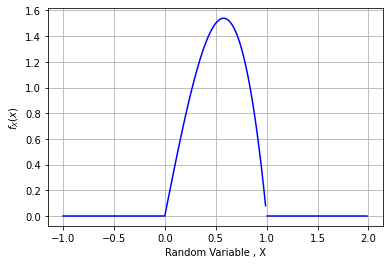
\includegraphics[width=.9\columnwidth] {Assignment_9_x.png}
    \caption{The marginal PDF of X}
    \label{fig:The PDF of X}
\end{figure}

\begin{figure}[!ht]
     \centering  
    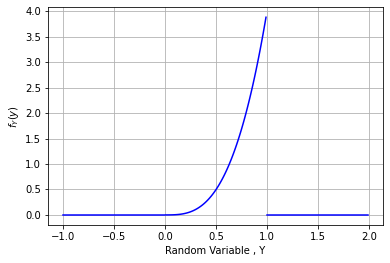
\includegraphics[width=.9\columnwidth] {Assignment_9_y.png}
    \caption{The marginal PDF of Y}
    \label{fig:The PDF of Y}
\end{figure}
\end{document}